%!TEX root = ../masters_thesis.tex

\chapter{Extensions} % (fold)
\label{cha:extensions}

This chapter evaluates the data model and the implementation developed in the previous chapter \ref{cha:development}. It focuses on the important aspects of the uncertain nature of history in section \ref{sec:evaluation}. The second part of this chapter \ref{sec:modelling_uncertainty} develops extensions to the Hivent Model and the Edit Mode for HistoGlobe that deal with these problems of uncertainty and disagreement.

% ==============================================================================
\section{Evaluation} % (fold)
\label{sec:evaluation}

In order to evaluate a model it is important to understand the concepts of \emph{disagreement} and \emph{uncertainty}, \emph{precision} and \emph{accuracy}. The model in an information system tries to resemble the real world as good as possible and necessary. Uncertainty and disagreement are two different kinds of problems in two different domains.
\emph{Disagreement} describes a conflict in the real world. On a contrary, \emph{uncertainty} is the imperfection of a model to describe the real world. Itcan be expressed by accuracy and precision: The better a model simulates the reality, the more \emph{accurate} or correct it is. That means, the closer it gets to the target, the higher is the accuracy. \emph{Precision} or exactness describes how similar the results of the model are compared to each other, independent from how well they resemble the real world. That means a precise model gets the same results over and over again (see figure \ref{fig:accuracy_precision}).

\begin{figure}[ht]
  \vspace{1em}
  \centering
  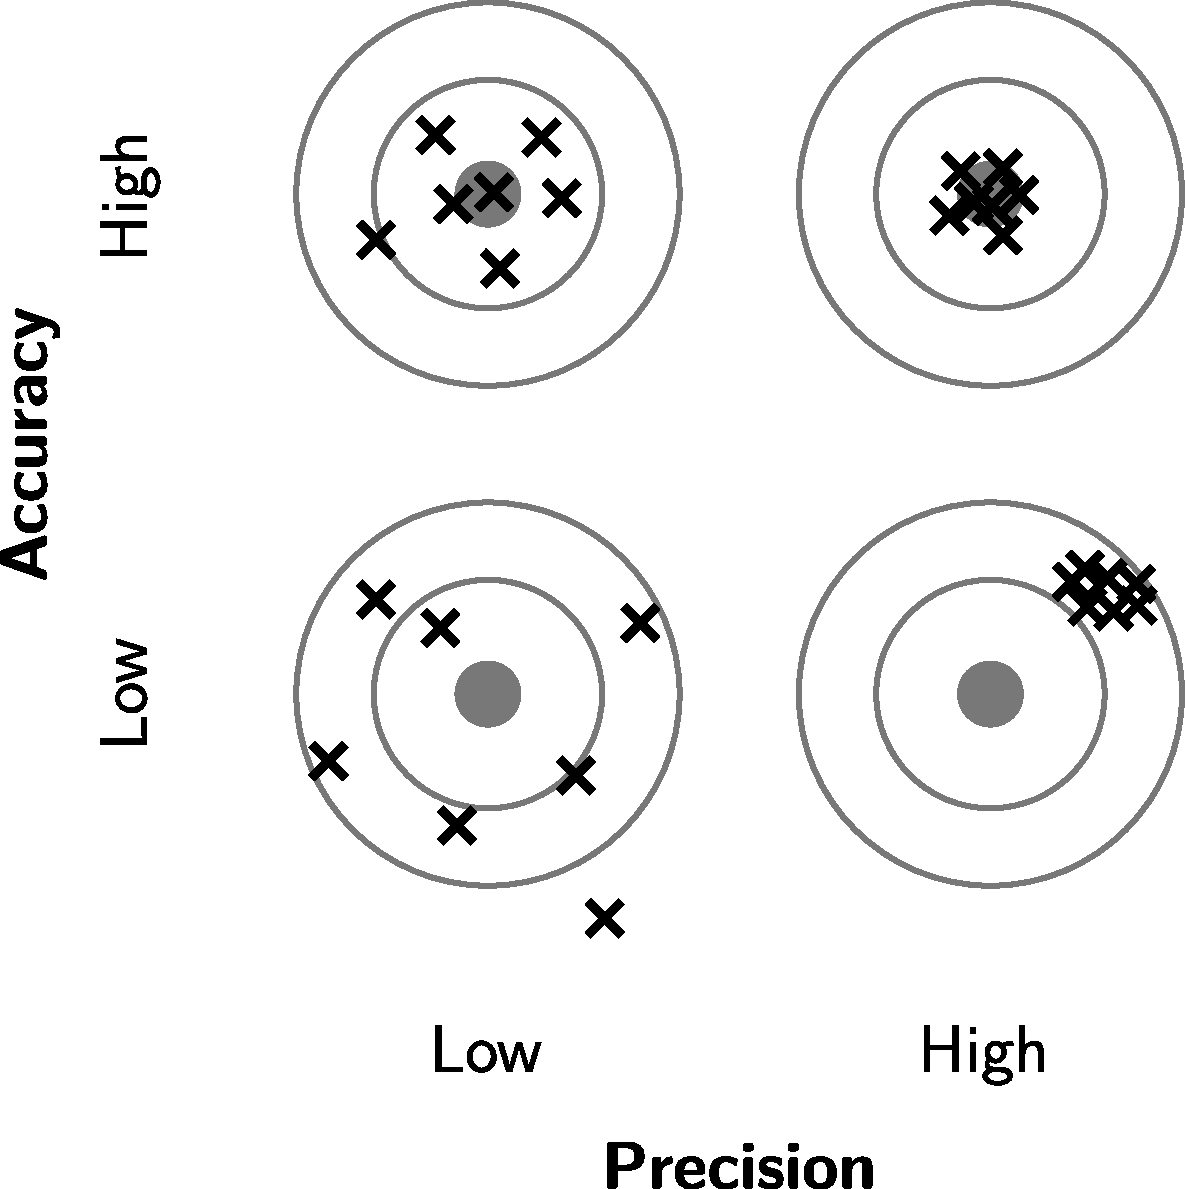
\includegraphics[width = 0.35\textwidth]{graphics/extensions/accuracy_precision}
  \caption{The difference between accuracy and precision}
  \label{fig:accuracy_precision}
\end{figure}


If the border between the Principalities of Transsylvania and Wallachia is deducted from an historical map of 1600, the course of that border is inaccurate to a certain degree, because the map does not show the real world correctly. However, it can be modelled in the system very precisely, because the coordinates of the border points are stored as floating point numbers.
The situation with Taiwan explained in section \ref{par:un_non_members_with_limited_recognition} is different: the disagreement is there already in the real world. The conflicting versions of the story can be modelled very precisely, but in order for the model to also be accurate, it needs to support declaring an Area as a contested territory.

% ------------------------------------------------------------------------------
\subsection{Analysis of the Data Model} % (fold)
\label{sub:data_model}

Each aspect of the Hivent Model proposed in section \ref{sec:hivent_model} is based on the prerequisite of full certainty of the data. The Hivent Model assumes that the dates of the Hivents, the names and territories of the historical and current Areas and the historical relations between Hivents and Areas are accurate and reasonably precise. However, this assumption is far from valid. Section \ref{sub:history_vs_geography} explained that in historical research, uncertainty is one of the major problems a historian has to deal with on a daily basis: primary sources can be biased towards the author, are certainly incomplete, inaccurate or conflicting with other sources. The acquisition of objective historical data is impossible. The further documents go back in time, the lower is the expected accuracy. Since all the information in the Historical Geographic Information System is based on primary sources, the data in the system inherits this integral lack of accuracy. This section evaluates the different components of the Hivent model in terms of how accurately and precisely they resemble the complex nature of history.

% - - - - - - - - - - - - - - - - - - - - - - - - - - - - - - - - - - - - - - -
\paragraph{Hivents} % (fold)
\label{par:evaluation_hivents}

The model contains the name, date and location of an Hivent. In reality, the name can have different versions: a long, official version and a short common version. The commonly known ``Treaty of Versailles'' is officially called the ``Treaty of Peace between the Allied and Associated Powers and Germany''. The name is different in other languages affected by the treaty. There can even be different versions of the name from different perspectives within the same language, e.g. the ``American Civil War'' was alternatively called ``War Between the States'', ``War for Southern Independence'' or ``War of Northern Aggression'' depending on the perspective.
The ~\texttt{Hivent}~ model does not account for different languages and versions and is therefore not very precise.

The ~\texttt{Hivent.date}~ is supposed to represent the temporal dimension of an historical event. While an historical change itself is discrete and happens at exactly one time point, the historical event yielding this change might not. The decisions of the ``Congress of Vienna'' came into effect on 9. June 1815, but the congress itself took place from September 1814 until June 1815. Another phenomenon becomes apparent in the ``Convention for the Extension of Hong Kong Territory'' (1898) which had a predefined length of 99 years. The treaty therefore has two dates in which historical changes happened: the date the treaty came into effect (Hong Kong becomes part of the United Kingdom) and the date it stopped being in effect (Hong Kong is handed over to China). Other interesting aspects are different calendar systems used in different parts of the world throughout history: the October Revolution in Russia (1917) happened in November in their Gregorian Calendar system, but in October in the Julian Calendar. Also timezones can play a crucial role: The German Instrument of Surrender ending World War II in Europe came into effect on 8. May 1945 at 23:01 Central European Time. In the Soviet Union that happened at 1:01 Moscow Time. That is why the celebration of the Victory Day in Moscow is celebrated on 9. May 1945. While the ~\texttt{Hivent.date}~ field in the data model works with timezones, it does not support different calendar systems or multiple dates associated with one ~\texttt{Hivent}~ which limits its precision.

The event location is represented by the ~\texttt{Hivent.location}~ name of a place, which can e.g. be a city, a battlefield or a region. The model is not very precise, because the actual geospatial location or region in which an historical event happened is not stored in the system. Additionally, it does not support names in different languages.

The Hivent model -- like any model -- is incomplete. There are relevant aspects about an historical event that are interesting for the purpose of the HGIS that are omittet in the model. In some cases the actors of an event are important, e.g. in a peace treaty. The model however doe snot answer the question ``Who?''. Even more severe is that there is no support of the most important question: ``Why'' something has happend. The motivation behind the actors or the coherences with other events are not supported in the model.

% paragraph evaluation_hivents (end)

% - - - - - - - - - - - - - - - - - - - - - - - - - - - - - - - - - - - - - - -
\paragraph{Areas} % (fold)
\label{par:evaluation_areas}

Also the model of an abstract Area, consisiting of a territory and a name, is problematic in terms of accuracy and precision. As it has been discussed in subsection \ref{sec:countries} in detail, it is impossible to objectively model a country without running into conflicts.
In the preconditions of the model it is fixed that there can not be overlapping territories at the same time -- although the nature of a contested territory is that it is claimed by more than one party. Whereas the data model allows to represent it as an own Area, it does not support any evidence of uncertainty about the status of an Area, e.g. being contested or international recognition.
The model does also not support hierarchies of Areas, e.g. countries within countries, provinces or overseas territories. Some parts of countries have varying degrees of autonomy which is also not supported by Areas in the Hivent Model.

The ~\texttt{AreaName}~ has the same problem than the ~\texttt{Hivent.name}, but it is more precise, because it contains both the formal and the short name of a country. However, uncertainty about the name, different versions or languages are not supported. More problematic is the ~\texttt{AreaTerritory}: The two assumptions in the preconditions of the Hivent Model in section \ref{sub:preconditions} -- constant coastline and no sea territory -- are inaccurate. The primary source for territories of countries are historical maps. The process of extracting a boundary from an historical map introduced in section \ref{par:historical_map} is error-prone and yields a loss of accuracy in each step. The level of inaccuracy depends on the resolution, map projection or the colors used in the map. In the data model it is not possible to provide information about the expected accuracy of a territory. Another problem is that the territory is stored as a whole polypolygon. Different parts of the border can have a different type or level of certainty status, e.g. one part a well-established and demarcated border to neighboring country $X$, but the border to neighbour $Y$ is contested. The ~\texttt{AreaTerritory}~ data model does not account for these differences.

% paragraph evaluation_areas (end)

% - - - - - - - - - - - - - - - - - - - - - - - - - - - - - - - - - - - - - - -
\paragraph{Hivent Operations} % (fold)
\label{par:hivent_operations}

Another aspect to evaluate is if the Hivent Operations as the basis of the spatio-temporal Hivent Model are collectively exhaustive, i.e. each possible case in the real world can be expressed with a combination of operations, and mutually exclusive, i.e. no operation can be replaced by a combination of two others \cite{mece}.

It is easy to see that a \texttt{NCH} operation is mutually exclusive to the other operations, because it is the only one that manipulates the name of an Area by preserving its identity. \texttt{UNI} and \texttt{SEP} are inverse, just like \texttt{INC} and \texttt{SEC} meaning that they are by the nature of an inverse exclusive. \texttt{INC} requires one update Area, multiple old Areas and no new Area, whereas \texttt{SEP} does not have an Area that preserves its identity and has several new Areas. Therefore \texttt{INC} and \texttt{SEP} are mutually exclusive, just like their inverse pair \texttt{UNI} and \texttt{SEC}.
Therefore, the only possible combinations left are \texttt{UNI} and \texttt{INC} and \texttt{SEP} and \texttt{SEC}. While both pairs are geographically equivalent, because they unite respectively separate the territory in the same way, they are historically distinct: \texttt{INC} and \texttt{SEC} hand model one update Area whose identity is preserved and territory updated while the others are incorporated into respectively secedes from this Area. In \texttt{UNI} and \texttt{SEP} on the other hand, there is no Area that is preserved. These two cases can not be mapped onto each other. Therefore it has been shown that all operations are mututally exclusive.

% TODO: show that is IS possible!
% idea: express UNI as INC + SEC at the same time, just like border change, but leaving no territory for one of the Areas => no SEC into $\Omega$ but directly into other Area. Would that work? If so, could we simplify everything by having only three Hivent Operations (INC, SEC, NCH) ?

To show that the collection of Hivent operation is exhaustive, all possible changes in the history of a country regarding its identity (formal name), short name and territory have to be examined. In reality, a historical country was once created, possible underwent several changes of its short name and territory and ceased one day. The creation of an Area on previously unclaimed land can be expressed by a \texttt{SEC} from $\Omega$. If it originated from one other Area, it is represented as the resulting Area of a \texttt{SEP}. If it had several predecessors, it is expressed by a \texttt{UNI}. However, the model does not support reincarnation, i.e. an Area continues the existance of another historical Area that has previously ceased. The data model is only geared to direct historical relationship. In the lifetime of the country, it can change its short name and its territory. A \texttt{NCH} operation enables the first case, an \texttt{INC} or \texttt{SEC} the second case. Since operations can be combined at the same point in time, all combinations of identity-preserving operations are possible. If a country ceases, it can either have none, one or multiple direct historical successors. The first case is represented by an \texttt{INC} into $\Omega$, the second case by a \texttt{UNI} and the third case by a \texttt{SEP}. Therefore, with the exception of reincarnation, all possible historical changes regarding the name and the territory of a country can be expressed with the Hivent Model.

% paragraph hivent_operations (end)

Overall, the Hivent Operations are a big strength of the Hivent Model, since it requires only five different operations.
The Hivent model also reasonably represents countries as Areas with a name and a territory. Countries with broad international recognition and a clear territory can be expressed without a problem. However, the model very poorly accounts for different levels of uncertainty in historical and geographic information: imprecise and inaccurate sources, different viewpoints and interpretations, contested territories, changing coastlines or different languages are not supported


% subsection data_model (end)

% ------------------------------------------------------------------------------
\subsection{Analysis of the Application} % (fold)
\label{sub:application}

Additionally to the data model, also the implementation of HistoGlobe can partially be evaluated. The interface resulted from a Human Centered Design process illustrated in chapter \ref{cha:development}. It underwent constant changes in multiple iterations with several user tests. Although there is a lack of quantitative data, the qualitative studies showed that both the Edit Operations and the interface as a whole were broadly understood. The only problematic operation was a border change: drawing the new territory of one Area and automatically adapting the other territory was not perceived as intuitive. As the name suggests, the users would have wished to actually change the border by editing the border points and moving it. Many users also complained that there is no feature to import existing geometries from external sources or from an historical map. While this is a highly desireable feature, it was out of the scope of this thesis but has a high priority in the future work.

In terms of performance system performs well with the current content of the database: It takes about 3.5 seconds to initially load all the data from the server to the client. As explained in section \ref{par:middleware}  all the data from the database is loaded at once. While this behaviour is not scalable, for the initial dataset it was sufficient: It took 3.5 seconds to load it. As soon as the amount of data in the database increases significantly, especially because of the territories, the approach to load all at once has to be changed to a gradual loading process: Initially the client sends the current date and the center of the viewport to the server. The server sends the currently active Areas close to the viewport center first. The goal is to minimize the time until the user sees a significant portion of the relevant data on the screen. This can also be achieved by storing different levels of detail of the vector data. Initially the server would send only the coarsest level to the client, then gradually increasing the granularity until the whole data is loaded on the client.

Given HistoGlobe would additionally to the current countries store a significant amount of historical countries since the beginning of the common era 2000 years ago. An estimation of the total memory consumption of the territories in the database is valuable. Currently there are about $200$ countries on Earth. Wikipedia lists another $700$ modern states in the ``List of former sovereign states''
\footnote{
  \emph{List of former sovereign states},
  \url{https://en.wikipedia.org/wiki/List_of_former_sovereign_states},
  last access: 02.06.2016
}
and additionally about $1000$ in lists of states of the Classical Age, Iron Age, Late Antiquity and the Middle Ages. However, some of them appear on several lists if the empires have existed throughout the Ages. As a broad estimate, there were probably not more than $1500$ historical ``countries'' since the beginning of the common era. Each of them probably underwent multiple territorial changes. The ``List of national border changes from 1815 to 1914''
\footnote{
  \emph{List of national border changes from 1815 to 1914},
  \url{https://en.wikipedia.org/wiki/List_of_national_border_changes_from_1815_to_1914},
  last access: 02.06.2016
}
collects about $75$ border changes, about $100$ border changes are listed since World War I. Therefore the estimation of $1$ international border change per year seems accurate. Given this rate of change stayed constant, there were about $2000$ border changes since the beginning of the common era. They are especially storage-intensive, especially because of the precondition with $\Omega$, each time the territory of one Area changes, at least one other will do so as well. As a conservative estimation, the total number of territories in the system will not exceed $2000 \times 2 + 1500 \approx 5000$. The current dataset of Natural Earth Data has a decompressed size of $8.8$ MB for about $200$ countries, that is about $0.05$ MB per country. Given that there would be accurate and precise measurements of all historical countries in the previous 2000 years, the total memory consumption for all coordinate data would not exceed $5000 * 0.05 \approx 250$ MB. That is an insignificant storage requirement and fits into the main memory of each modern computer system.

% subsection application (end)

% section evaluation (end)

% ==============================================================================
\section{Modelling Uncertainty} % (fold)
\label{sec:modelling_uncertainty}

The first part of this chapter presented a list of shortcomings of the current Hivent Model and the implementation, most of them focussing on the problem of undcertainty and disagreement. The purpose of this section is to develop approaches to increase the accuracy of the model with respect to uncertainty. A higher accuracy usually leads to a higher complexity of the data model. This trade-off has to be thoroughly taken into consideration when supporting a new feature. For that reasons some problems are be ignored in the rest of this chapter:

\begin{itemize}
  \item The preconditions of the Hivent Model will not change, i.e. countries will stop on their coastlines and the distribution of water on the planet has not changed in history -- otherwise the model would need to support not just sudden events but also gradual processes. This out of the scope of the thesis.
  \item The support for different historical perspectives on the same Hivent, e.g. different names and descriptions or even different historical changes would create a research tool with great potential. It would enable the possibility for different versions of history based on alternative scenarios: ``What if X would have (not) happened?''. However, this would significantly increase the complexity of the system and would also be very subjective.
  \item The introduction of different calendar systems would not increase the accuracy of the model significantly. The dates in the system must all stick to the Julian calendar, which is a reasonable requirement to avoid unnecessary complexity.
\end{itemize}

In order to tackle the remaining shortcomings of the current concept, both the user interface and the data model have to be extended. The main problem when dealing with uncertainty is that from the perspective of a computer, there is no such thing as an uncertain value of a variable. That is why all sorts of uncertainty must ironically be quantified: The computer needs to know exactly how uncertain the user is about the data.

% ------------------------------------------------------------------------------
\subsection{International Recognition} % (fold)
\label{sub:international_recognition}

\begin{figure}[ht]
  \centering
  
\includegraphics[width = 0.6\textwidth]{graphics/extensions/edit_mode_extension.png}
  \caption{Newly designed and extended buttons for Edit Operations.}
  \label{fig:edit_mode_extension}
\end{figure}

Two new Edit Operations shown in figure \ref{fig:edit_mode_extension} are introduced: \texttt{CHS} changes the status of an Area and \texttt{REC} declares a new recognition, i.e. one country internationally recognizes another one. This is simply performed by selecting two Areas on the map, whereas the first Area recognized the second.

\begin{figure}[ht]
  \centering
  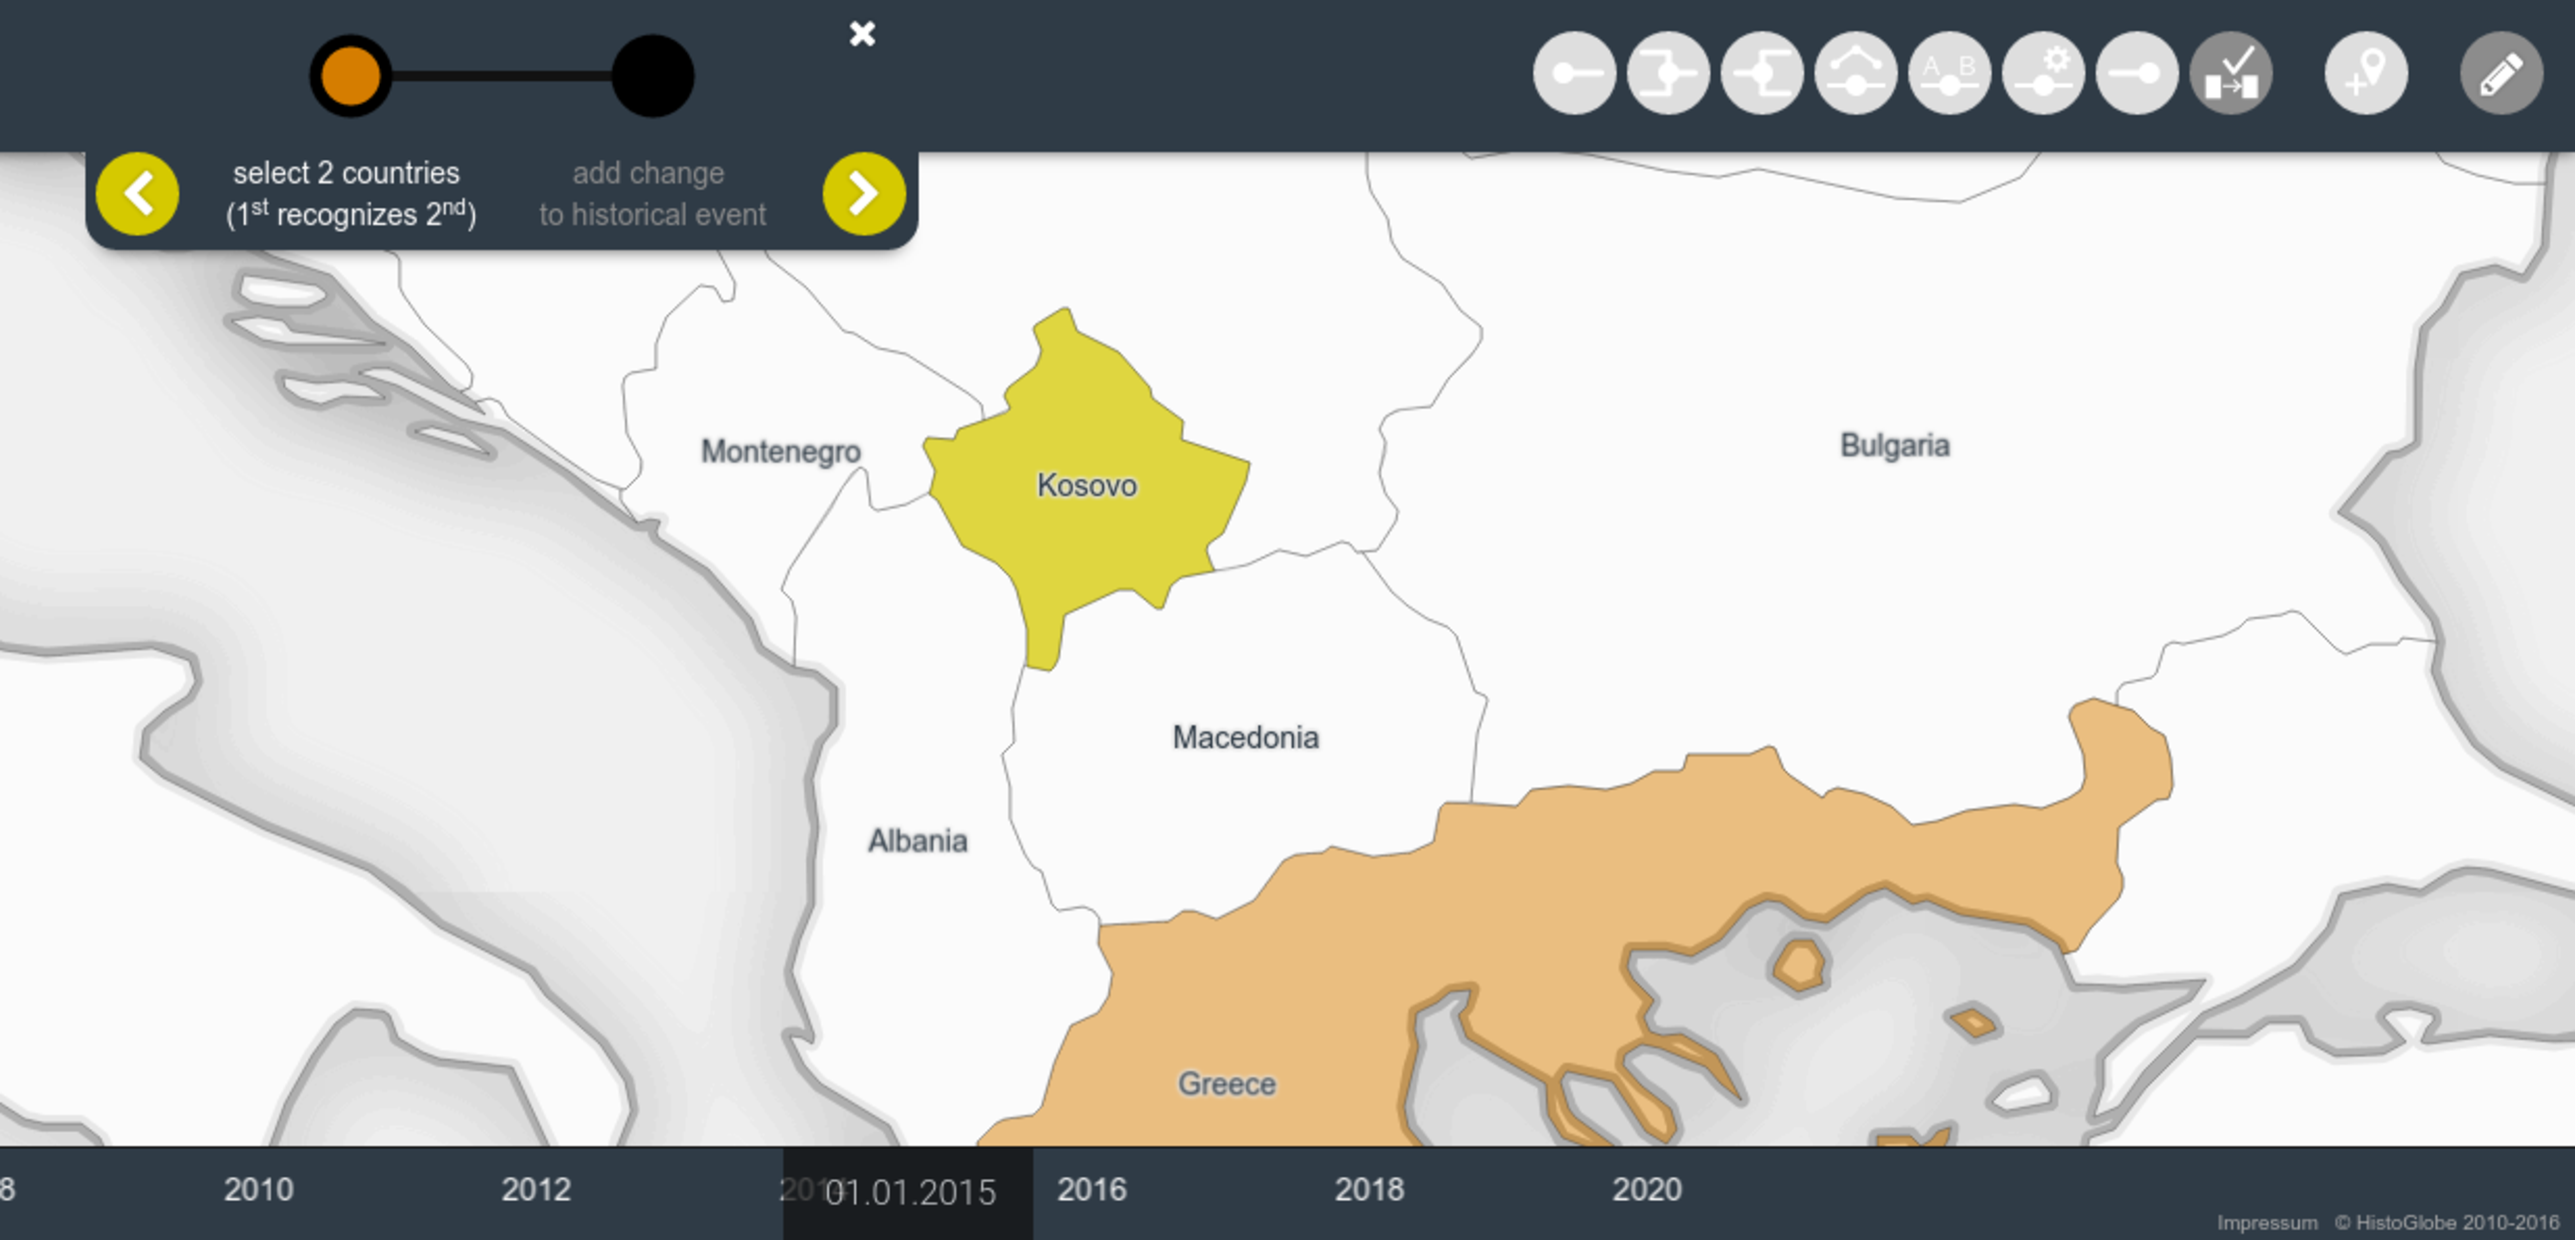
\includegraphics[width=0.6\textwidth]{graphics/extensions/operation_REC}
  \caption{New Edit Operation: Recognition -- sets up the recognition of one Area to another.}
  \label{fig:uncertainty_operation_REC}
\end{figure}

% subsection international_recognition (end)

% ------------------------------------------------------------------------------
\subsection{Uncertain Borders} % (fold)
\label{sub:uncertain_borders}

Also the Edit Operation workflow is altered. The second step \texttt{SetNewTerritories} defines the territory of the new Area(s). Instead of drawing the whole territory as a set of polygons, the user draws one borderline at a time, geometrically as a polyline. This has the main advantage that each part of the border is treated separately. The borderline is assigned a degree of certainty, in the interface controlled by a horizontal slider, in the model as a certainty value (\texttt{certainty} $\in~]0 .. 1]$). Absolute certainty ($1.0$) creates a sharp and crisp line on the map. In case of uncertainty (\texttt{certainty} $\in~]0..1[$) three different visualization methods are introduced:

\begin{enumerate}
  \item Blurred Border: The higher the uncertainty, the wider and more blurry the border.
  \item Border Corridor: With increasing uncertainty, the offset around the actual border line extends. That creates a corridor in which the actual border is probably in.
  \item Blurred Border Corridor: The combination of the first two approaches.
\end{enumerate}

A simple model for the calculation of the blur factor, line width and offset distance is:
\begin{center}
\begin{math}
    f(c) = -1 \cdot S \cdot ln(c) + I
\end{math}
\end{center}
where $c$ is the certainty factor, $S>0$ is a scaling factor and $I$ is the inital value (for width: $1~px$, for blur: $0$, for offset: $0~px$). In the example in figure \ref{fig:uncertainty_border} the scaling factor is $S=4$. In the Blurred Border Corridor method, the scaling factor for line width and the blur factor was halved. Further analysis and user testing are required in order to decide for one approach to develop further.

\begin{figure}[ht]
  \vspace{1em}
  \centering
  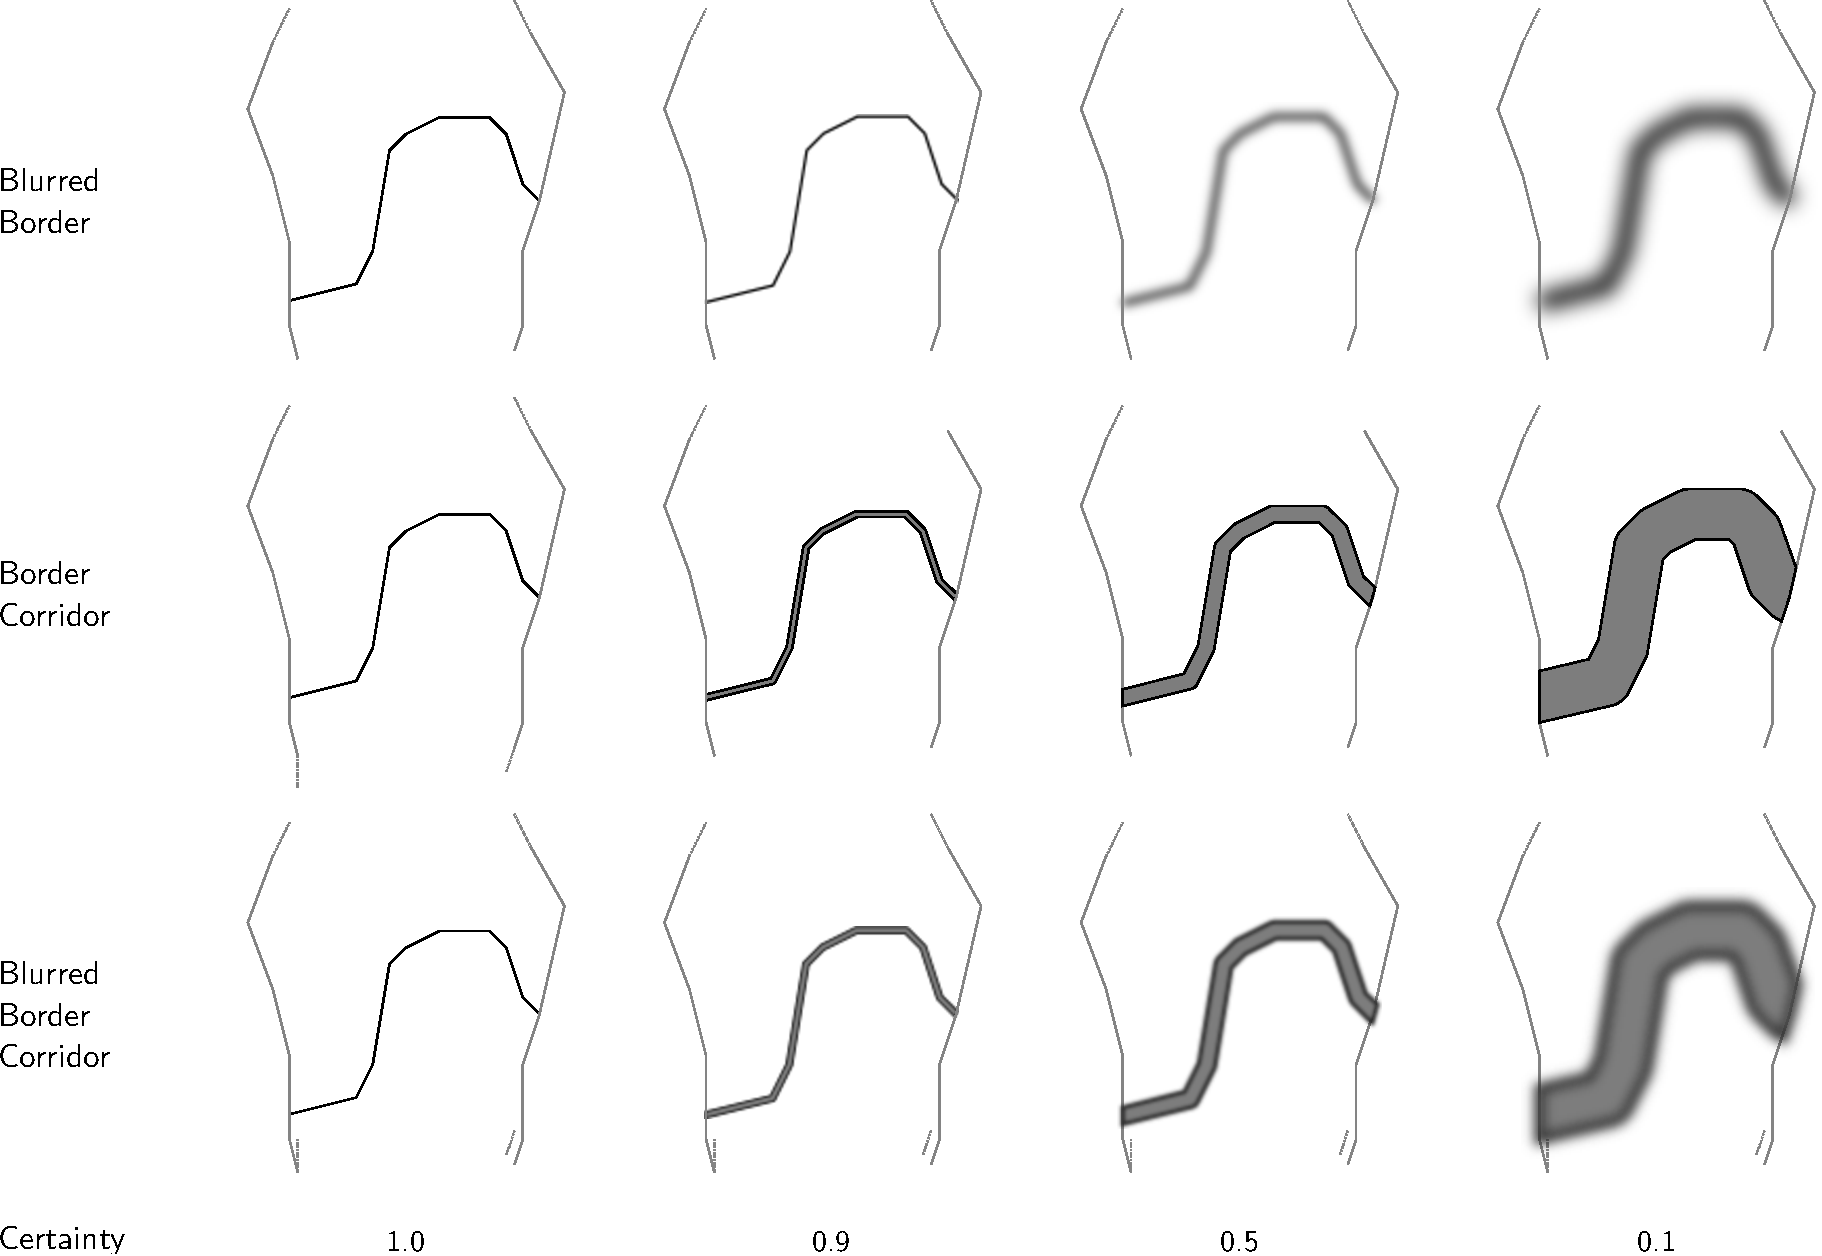
\includegraphics[width = 0.8\textwidth]{graphics/extensions/border}
  \caption{Three different methods to visualize uncertain courses of a border}
  \label{fig:uncertainty_border}
\end{figure}

Another advantage of the input of borderlines instead of territories is that once the model is further advanced, coastlines can be continuously changed according to an appropriate change model. This can be applied solely to the coastlines without affecting the interior borders.

A new border point automatically snaps to an existing border point, if the mouse position is close enough to it (an appropriate threshold might be $5~px$). This allows for a smooth workflow and is required to create closed polygons. When the user finished a territory by defining all surrounding polylines that create a closed ring, the polygon is assembled. If a borderline meets another borderline at an interior node, the polyline splits up into two parts so that each meeting point of borders is the start or end point of a polyline. This way the spatial integrity is maintained.

\begin{figure}[ht]
  \vspace{1em}
  \centering
  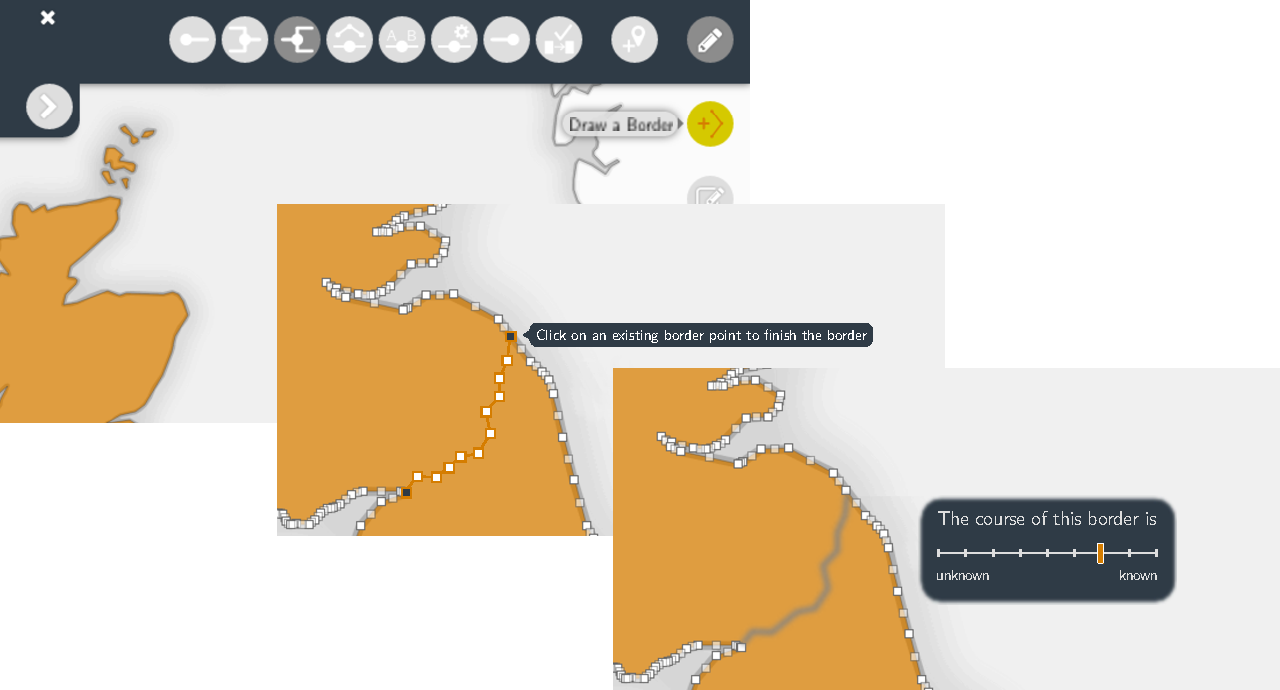
\includegraphics[width = 0.8\textwidth]{graphics/extensions/new_territory_tool}
  \caption{Drawing historical borders instead of full Areas and definining a level of certainty.}
  \label{fig:uncertainty_new_territory_tool}
\end{figure}

If the created territory overlaps with an existing territory, its intersection will created a separate territory. In the next step, this territory can then be defined as a contested Area or defined as a part of another Area. If the step yields an empty territory that was claimed before, it can later be defined as a neutral zone or unclaimed land.

% subsection uncertain_borders (end)

% ------------------------------------------------------------------------------
\subsection{Special Areas} % (fold)
\label{sub:special_areas}

To treat special Areas differently, a new step in the workflow is defined. After the territory and the name of a new Area have been defined, a special status can be assigned to it.

\begin{enumerate}
  \item A \emph{fully sovereign country} is a political entity with full sovereignty over its territory and people and significant international recognition, e.g. Estonia.
  \item An \emph{unclaimed land} is a territory that is not claimed by any political entity, e.g. Antarctica.
  \item A \emph{neutral zone} is often a buffer zone between two conflicting parties, e.g. currently on Cyprus.
  \item A \emph{contested territory} is claimed by at least two different political entities of the same hierarchical level, e.g. the Kashmir region between India and Pakistan. It is also suitable for Areas that have claimed independence from a sovereign country but are not yet regonized as such, making their whole territory contested, e.g. Nagorno-Karabakh (see figure \ref{fig:uncertainty_new_status_tool}).
  \item A territory can be a subordinate part of another country with a certain degree of autonomy ($\in [0..1]$). Fully subordinate parts of a country, like a US State or a German Bundesland have no autonomy ($0$). Autonomous countries within another country, like England to the United Kingdom or Greenland to Denmark, receive have certain a degree of autonomy ($\in ]0..1[$). The value $1$ is excluded, because full autonomy means the territory is a sovereign country.
\end{enumerate}

\begin{figure}[ht]
  \centering
  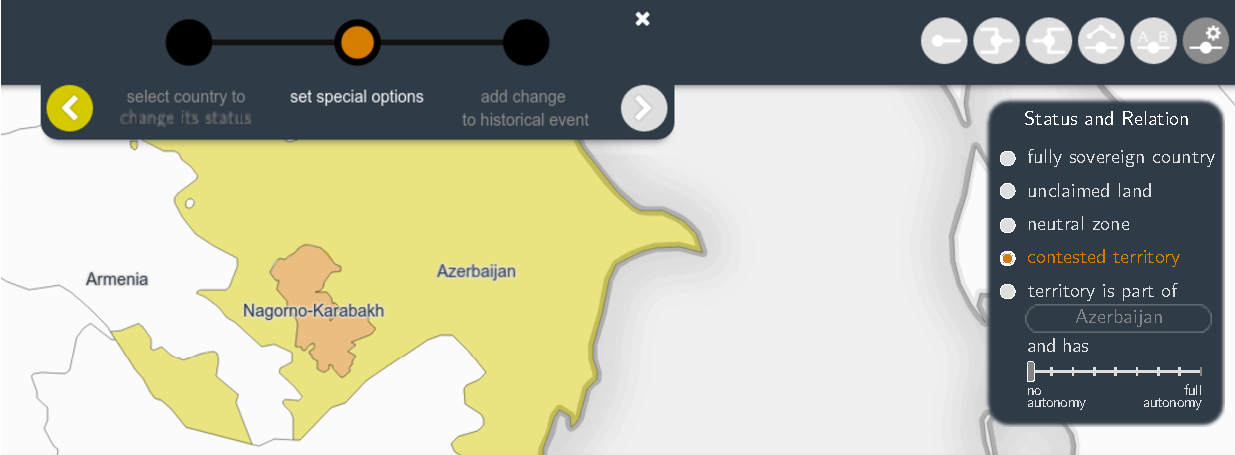
\includegraphics[width = 0.8\textwidth]{graphics/extensions/new_status_tool}
  \caption{Defining a special status or relationship to a territory.}
  \label{fig:uncertainty_new_status_tool}
\end{figure}


% subsection special_areas (end)

% ------------------------------------------------------------------------------
\subsection{Content from Wikipedia} % (fold)
\label{sub:content_from_wikipedia}

As it has been envisioned in section \ref{sub:data_sources}, Wikipedia stores a lot relevant data for HistoGlobe which is not straightforward to reuse, because of the Hivent-based data model and the lack of broad standardization in Wikipedia. This section assumes that the data could be parsed and processed easiliy. When defining the name of an Area, the user will get actual name suggestions from a collection of current and historical countries in Wikipedia. That saves time for researching short and formal names of Areas.

\begin{figure}[H]
  \centering
  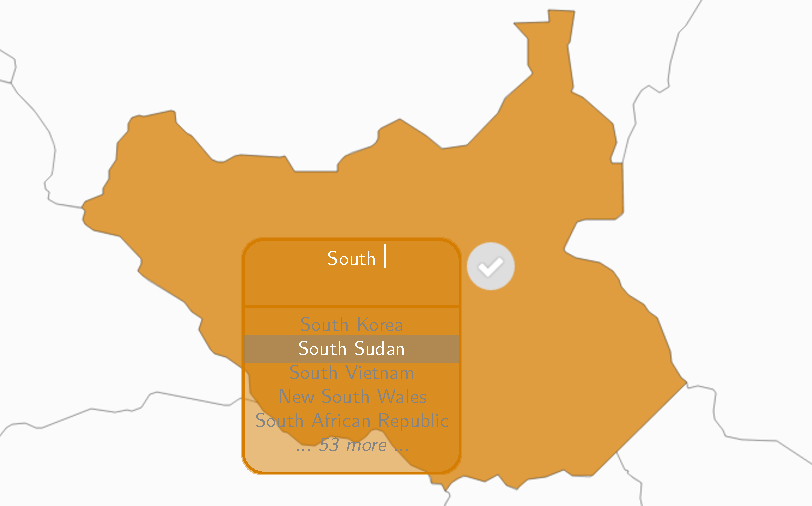
\includegraphics[width=0.5\textwidth]{graphics/extensions/new_name_tool}
  \caption{Getting suggestions for the name name from Wikipedia.}
  \label{fig:uncertainty_new_name_tool}
\end{figure}

% - - - - - - - - - - - - - - - - - - - - - - - - - - - - - - - - - - - - - - -
\newpage
\paragraph{New Hivent Box} % (fold)
\label{par:new_hivent_box}

The visualization of an Hivent is split up into three parts (see see figure \ref{fig:uncertainty_new_hivent_box}):

\begin{enumerate}
  \item An information section storing important meta data of the event location, the dates (timespan in which the event happened), a description and the lin kto the wikipedia article (if given).
  \item A section storing all Edit Operations associated with that Hivent. Each operation is visualized and is assigned a date at which this event came into effect.
  \item A multimedia section stores images, videos, audio files and documents and their sources associated to the historical event.
\end{enumerate}

Similar to the extension of the Area name step, also Hivent names can be chosen among a collection of Wikipedia articles describing historical events. Selecting a name from a wikipedia article automatically fills the information section and adds multimedia files from the wikipedia article. The Edit Operation is automatically entered in the section. With this separation, different Edit Operations at different dates can be associated with one Hivent, increasing the accuracy and precision of the Hivent Model.

\begin{figure}[ht]
  \centering
  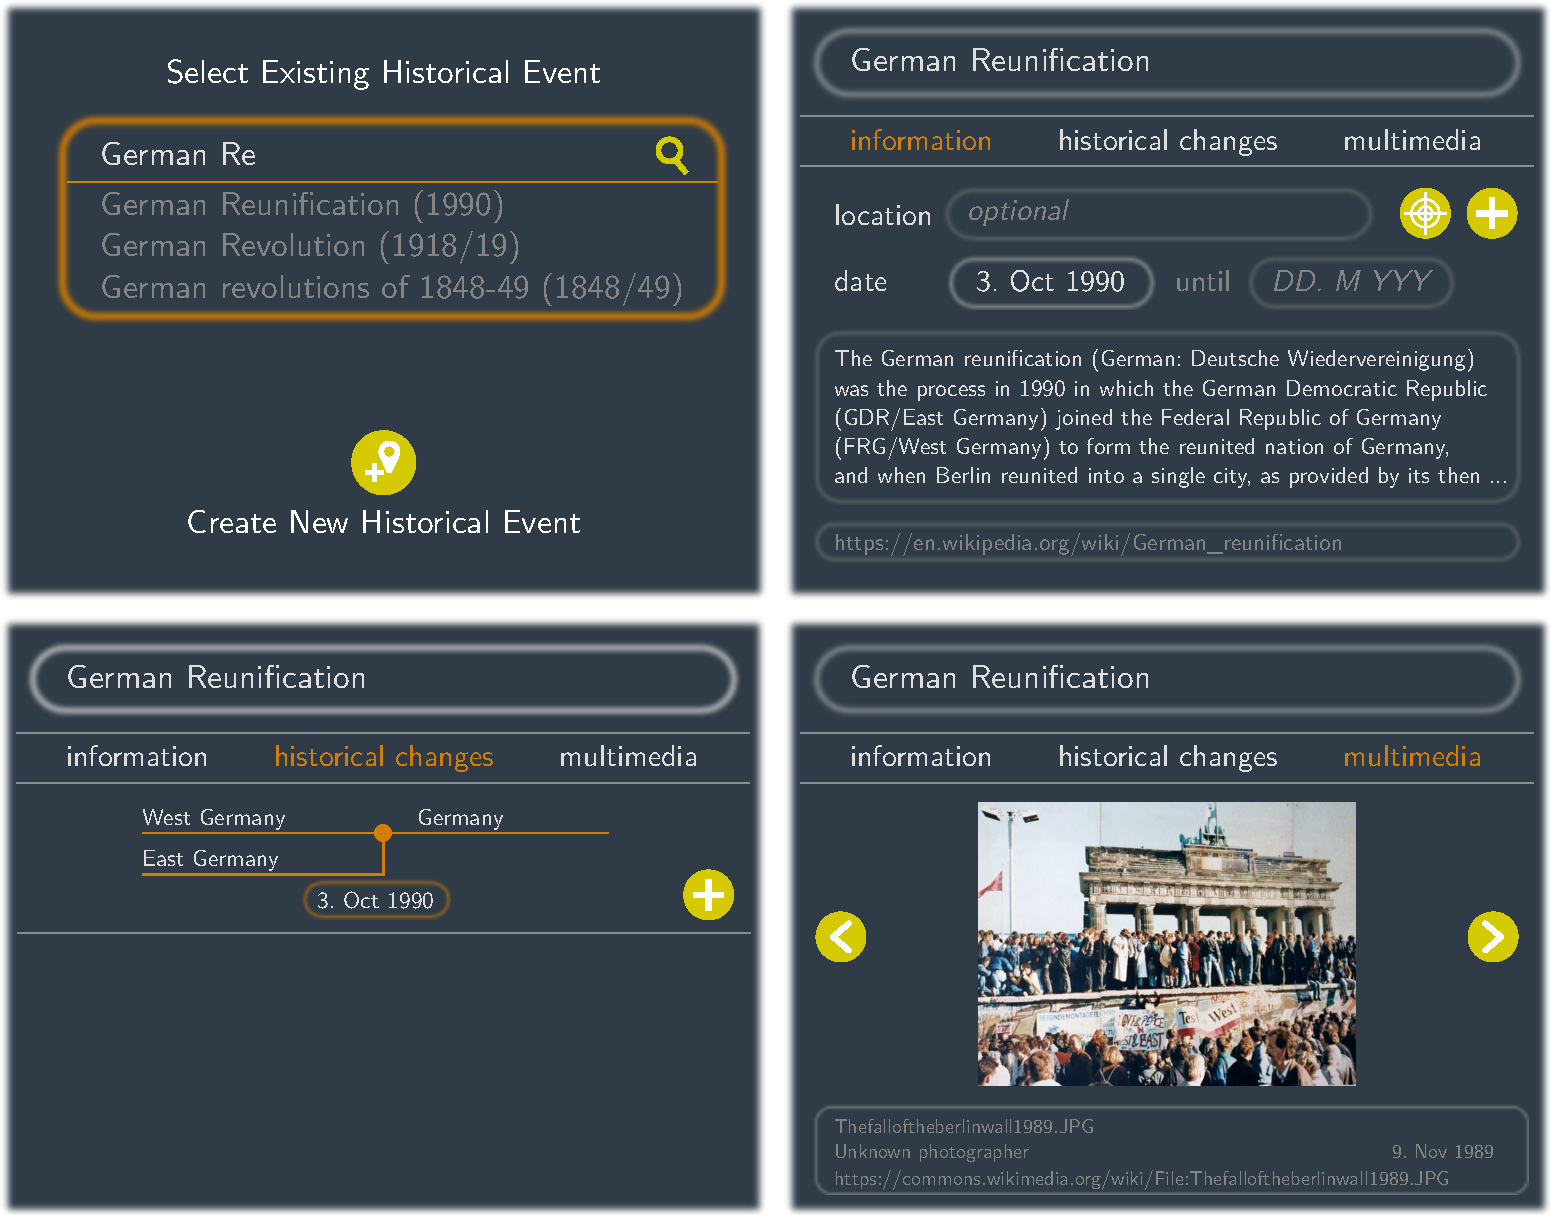
\includegraphics[width = 0.8\textwidth]{graphics/extensions/new_hivent_box}
  \caption{Creating a new Hivent and adding the newly created Edit Operation.}
  \label{fig:uncertainty_new_hivent_box}
\end{figure}

In the long run, HistoGlobe can be synchronized with Wikipedia or even be designed as an extension for Wikipedia articles about current or historical countries.

% paragraph new_hivent_box (end)

% % - - - - - - - - - - - - - - - - - - - - - - - - - - - - - - - - - - - - - - -
% \paragraph{Multi-language support} % (fold)
% \label{par:multi_language_support}

% In order to support different languages, a language selection is placed on the bottom right corner of the interface, on the timeline. This changes the language of the whole interface and loads the translations of the Area names and the Hivent names, locations and descriptions in the newly created language. If a term is not defined in the language, the fallback language (English) is used instead.

% \begin{figure}[ht]
%   \centering
%   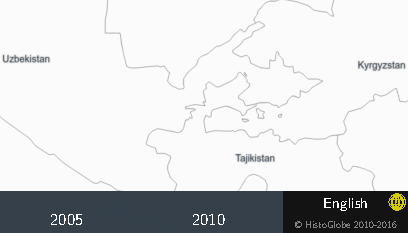
\includegraphics[width = 0.45\textwidth]{graphics/extensions/multi_language}
%   \caption{Changing the language in the user interface.}
%   \label{fig:multi_language}
% \end{figure}

% paragraph multi_language_support (end)

% subsection content_from_wikipedia (end)

% ------------------------------------------------------------------------------
\subsection{Extended Hivent Model} % (fold)
\label{sub:extended_hivent_model}

To account for the extensions in the interface, also the data model has to be adapted. Mainly the thematic domain of the Hivent Model changed, since the status or an Area, its recognition or relation to other countries is a non-spatial attribute of the data. The new Edit Operations that were introduced need to be internally  expressed by Hivent Operations. For that purpose the name change operation (\texttt{NCH}) is abstracted to a thematic change operation (\texttt{TCH}). Instead of changing only the \texttt{old\_name} to the \texttt{new\_area} of its associated update Area, it can also change its \texttt{old\_status} to a \texttt{new\_status}. It can be visualized in exactly the same way, since it is just as well an identity-preserving change.

More thoughts have to be spent on the question how to express a new recognition of an Area in an Hivent Operation. Additionally, the introduction of hierarchical layers of Areas adds new requirements to the Hivent Model: All Hivent Operations can potentially be performed on the same level of hierarchy as before, but also downwards or upwards. The example of the fictional secession of Scotland from the United Kingdom in 2018 would be simple: The user could simply select Scotland as a second-level Area inside the first-level United Kingdom and secede Scotland from the Union by updating its status to a fully sovereign first-level Area. The design and implementation of the data model requires further analysis.

\begin{figure}[ht]
  \vspace{1em}
  \centering
  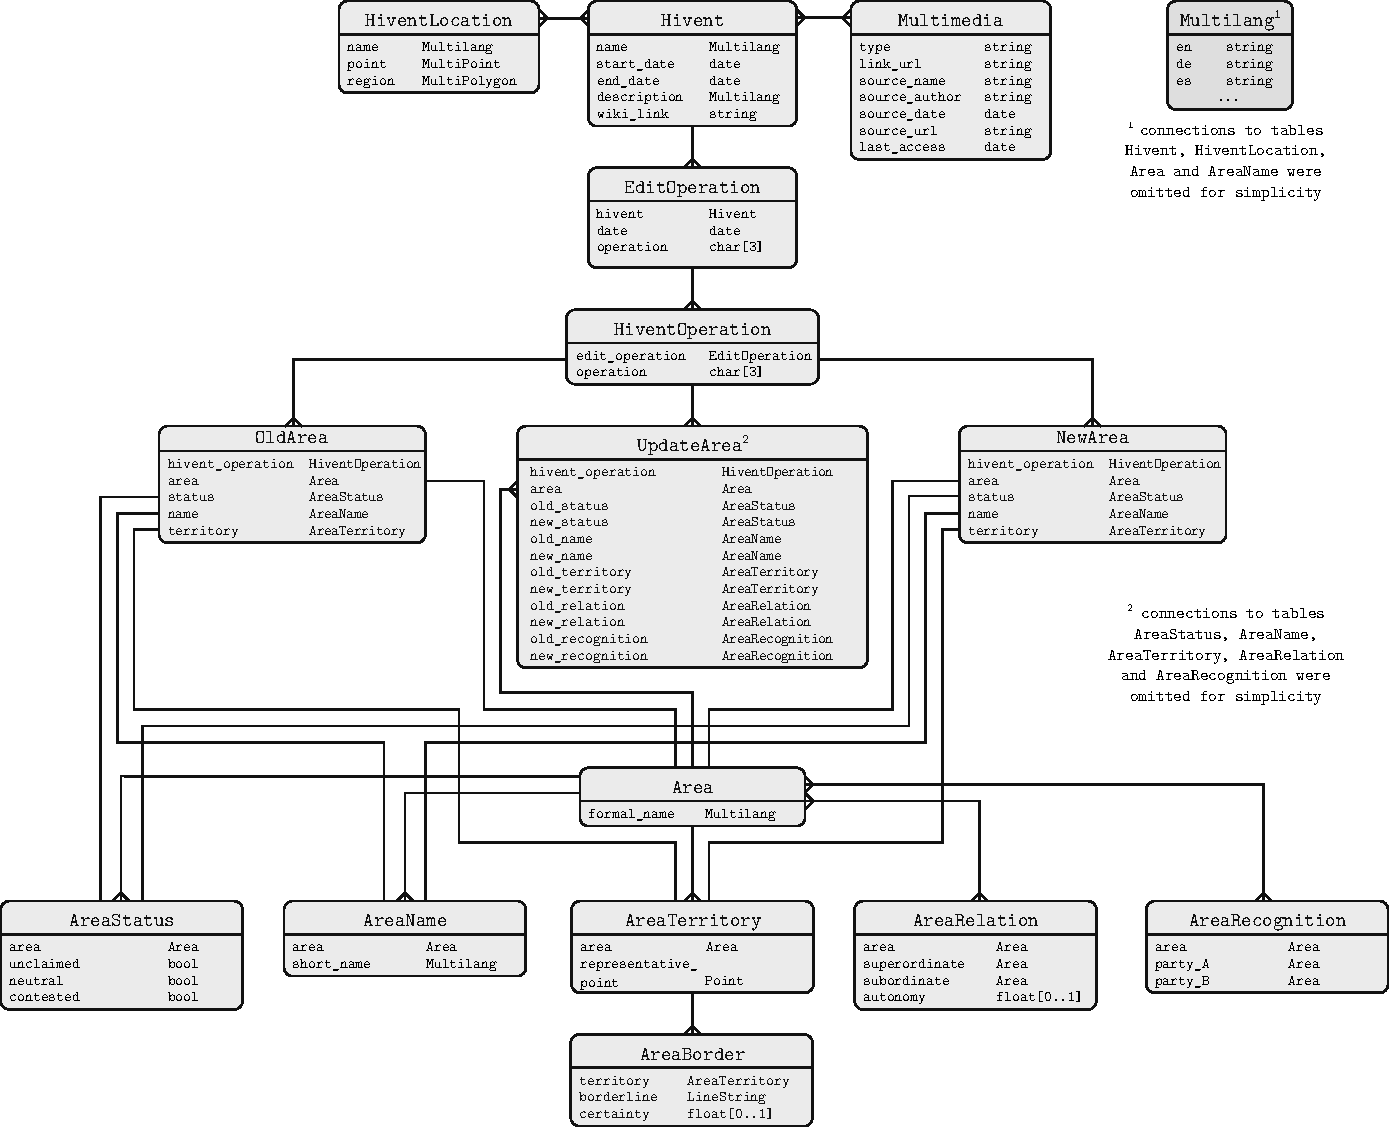
\includegraphics[width = 0.8\textwidth]{graphics/extensions/new_database_model}
  \caption{The new data model to support the developed approaches regarding uncertainty}
  \label{fig:new_data_model}
\end{figure}

The Hivent database model from section \ref{sub:server_side_application} is extended by the following entities and relations:

\begin{enumerate}
  \item Creation of a \texttt{Multilang} entity to store a name of an Hivent, its location or an Area name in different languages.
  \item Outsourcing of the \texttt{HiventLocation} into an own entity to identify a location with a name and a geospatial reference.
  \item Creation of a \texttt{Multimedia} entity to manage multimedia files associated to an Hivent.
  \item Attachment of a date to an \texttt{HistoricalChange}.
  \item Inclusion of the \texttt{formal\_name} into the \texttt{Area} to emphasize it as the identifier.
  \item Creation of an \texttt{AreaBorder} with a \texttt{borderline}. A set of \texttt{AreaBorders} create one \texttt{AreaTerritory} which is associated to the Area. Each change of an \texttt{AreaBorder} creates one or two new \texttt{AreaTerritory}/ies.
  \item Creation of an \texttt{AreaStatus} an an \texttt{AreaRelation} to account for special status of an Area alone or in relation to another Area with a certain level of autonomy.
  \item Creation of an \texttt{AreaRecognition} to account for international recognition of one Area to another one.
  \item Adaption of the \texttt{AreaChange} entity to model a change of each possible property of an Area.
\end{enumerate}

% subsection extended_hivent_model (end)

% section modelling_uncertainty (end)

% chapter extensions (end)

% ==============================================================================

\vspace{2em}

This chapter provided an analysis of the data model and the implementation developed in the previous chapter. The main problem with the current state of the application is that it does not support any kind of ways to cope the inherent problem of uncertainty and disagreement in history. For of the shortcomnings from the evaluation design solutions for the user interface of HistoGlobe were developed and integrated into the Hivent Model. The final chapter of this thesis summarizes the achievements of this and the previous chapter, embeds the work into the current state-of-the-art and concludes the thesis as a whole.